\subsection{토큰화}
\label{sec:tokenisation}


모든 것을 텍스트로 다루는 표준 LLM과 달리, 금융 파운데이션 모델은 표 형식(tabular) 데이터의 구조적 성격과 이질성을 보존해야 한다.
저자들은 이 문제를, 입력 토큰의 의미 구성요소가 분리된(disentangled) 임베딩 공간을 도입해 해결한다.

그림~\ref{fig:tokenisation}에서 볼 수 있듯, 저자들은 표 형식 이벤트 데이터의 일반 표준에 따라~\citep{braithwaite2025your} 각 데이터 포인트를 세 가지 구성요소로 표현한다 — 의미 타입(키), 값, 시간 좌표.
예를 들어, \texttt{Channel:} \texttt{email} at \texttt{24-04-07 19:20:18}은 각각 키, 값, 시간 좌표로 매핑된다.
이는 모델이 필드의 의미와 값을 구분해서 다루도록 보장하면서, 이벤트의 시간 순서까지 함께 인코딩한다.
이어서 세 구성요소가 어떻게 토큰화되는지 차례로 설명한다.

\begin{figure}
    \centering
    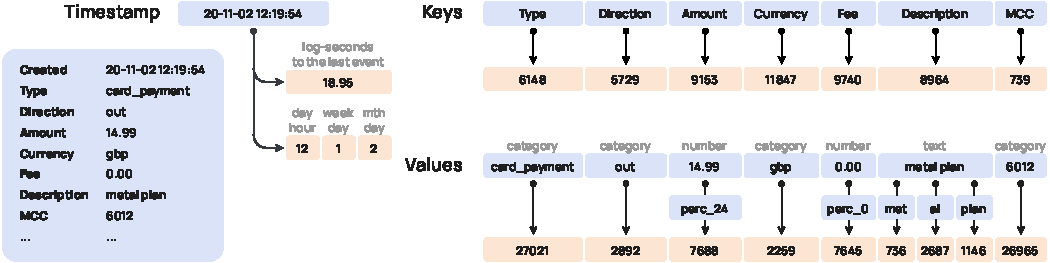
\includegraphics[width=1\linewidth]{images/tokenisation.pdf}
    \caption{
        \textbf{토큰화 개요}.
        원시 이벤트 레코드는 시간 좌표, 의미 타입(키), 값으로 분해된다.
        키는 항상 하나의 토큰으로 표현되고, 값은 타입별 토큰화를 따른다 — 수치값은 백분위 버킷으로, 범주값은 하나의 토큰으로, 텍스트 값은 서브워드 토큰들로 분해된다.
        따라서 어떤 키는 여러 개의 값 토큰으로 펼쳐지기도 한다(예: \texttt{Description} $\rightarrow$ \texttt{met}, \texttt{al}, \texttt{plan}).
        시간은 직전 이벤트까지의 로그-초(log-seconds)와, 타임스탬프에서 유도된 달력·시간 피처로 함께 인코딩된다.
        프로필 상태는 이벤트 레코드와 비슷하게 인코딩된다.
    }
    \label{fig:tokenisation}
\end{figure}

\paragraph*{의미 타입(키).}
의미 타입 임베딩은 모델이 각 필드의 의미를 학습하고 그 값을 맥락에 맞게 해석할 수 있도록 해 준다.
저자들은 모든 의미 타입(키)을 단일 토큰으로 토큰화하며, 이벤트와 프로필 상태의 의미 타입을 동일한 방식으로 인코딩한다.
그 결과 약 60개 토큰 규모의 어휘가 만들어진다.

\paragraph*{값.}
저자들은 값의 다양성을 \emph{수치형}, \emph{범주형}, \emph{텍스트형}의 세 가지 값 타입으로 다룬다.
수치값은 백분위(percentile) 버킷으로 매핑되며, 버킷 경계는 학습 데이터에서 학습되고 0을 위한 별도 버킷이 추가되며, 각 버킷마다 토큰을 하나씩 할당한다.
범주형과 텍스트형의 구분은 카디널리티 임계화(cardinality thresholding)로 정해진다 — 고유값 개수가 미리 정한 임계 미만인 문자열 필드는 범주형으로, 그보다 큰 필드는 텍스트형으로 다룬다.
범주값은 가맹점 카테고리 코드(MCC) 같이 자주 등장하는 값이 여러 토큰으로 쪼개지지 않도록 모든 텍스트 필드에서 수동으로 선정되며, 마찬가지로 단일 토큰으로 표현된다.
텍스트 필드의 값은 BPE(Byte-Pair Encoding) 스타일 서브워드 토크나이저(subword tokeniser)로 토큰화되며~\citep{sennrich2016neural}, 드문 미관측 조각을 위해 \texttt{[UNK]} 토큰이 따로 예약된다.
값 전체 어휘 크기는 약 28\,k 토큰이다.

\paragraph*{시간 정보.}
저자들은 시간을 두 가지 방식으로 인코딩한다.
첫째, 가장 최근 이벤트로부터 경과한 시간을 초 단위로 계산한다.
이어서 부드러운 로그 변환 $8\cdot\ln(1+t/8)$ 을 적용해, \emph{라이프롱} 이벤트의 동적 범위를 압축하면서도 최근 이벤트에 대해서는 고해상도의 선형 세분성을 유지한다.
이는 극단적인 시간 간격 때문에 위치 임베딩(positional embedding)에서 발생할 수 있는 앨리어싱(aliasing)을 막으면서도, 가까운 이벤트의 순서 정밀도는 희생하지 않게 해 준다.
둘째, 일간·주간 시간 주기를 포착하기 위해, 각 이벤트 타임스탬프를 시각의 시(hour of day), 요일(day of week), 일자(day of month)로 분해하고, \citet{gorishniy2022embeddings}와 비슷한 주기 함수로 임베딩한다. 다만 주기는 학습되는 대신 알려진 달력 주기로 고정한다.
달력 피처는 이벤트 이력 항목에만 적용된다. 일회성 라이프롱 이벤트에서는 로그-초 인코딩만으로도 관련 시간 신호를 충분히 담을 수 있어, 주기 패턴이 덜 중요하기 때문이다.
